\documentclass[12pt]{report}
\usepackage[utf8]{inputenc}
\usepackage{graphicx}
\usepackage{subcaption}
\usepackage{makecell}
\usepackage{array, booktabs, caption}
\usepackage{amsmath}
\usepackage{amsfonts}
\usepackage{amssymb}
\usepackage{multirow}
\usepackage{csquotes}
\usepackage{longtable, booktabs}
\usepackage{siunitx}
\usepackage{algorithm}
\usepackage{tabularx}
\usepackage{algpseudocode}
% Custom Macros
\algnewcommand\algorithmicforeach{\textbf{for each}}
\algdef{S}[FOR]{ForEach}[1]{\algorithmicforeach\ #1\ \algorithmicdo}

\includeonly{chapters/chapter04}
\graphicspath{ {images/} }

\title{
    {Fine-Grained Activity Detection in the Kitchen with UWB}\\
    {\large University of Alberta}\\
    {
\includegraphics[width=\textwidth]{university.png}}
}
\author{Steven Phan}
\date{08 April 2023}

\begin{document}
\maketitle

% ==================================================
% PREWORD

% \chapter*{Abstract}
% This is my abstract
% \chapter*{Dedication}
% to someone
% \chapter*{Declaration}
% i declare that..
% \chapter*{Acknowledgements}
% I want to thank....
\tableofcontents

% ==================================================
% CHAPTERS
\chapter{Introduction}
This thesis project investigates how to detect fine-grained action within the meal preparation activity of daily living 
(ADL) in the home without the use of privacy-intruding cameras. ADLs are common activities that an individual 
performs inside their homes. These include walking around, eating, dressing, personal hygiene, toileting, 
transportation, meal preparation, house cleaning, and managing medication. The meal preparation ADL was chosen as the 
main focus because cooking is a uniquely enjoyable activity while being procedurally dense. 
% TODO: find something that says that cooking is cognitively challenging. Or is cognitively and physically demanding
Meal preparation can include 
the following actions: opening the fridge, retrieving ingredients, cutting vegetables, and assembling the ingredients. 
Monitoring these actions may be used as part of a health monitoring program by enabling the assessment of the presence, 
duration, and correctness of each individual step in a goal-orientated activity. Missing or incorrect steps can be indicative of 
forgetfulness, and steps that take a long time can be indicative of low-efficacy or struggle that clinicians can address.
Information obtained through the monitoring of the cooking task may help guide interventions 
and track the effectiveness of interventions in clinical populations such as people with dementia, and frailty. 
A further and more in-depth review of the background will be done in Chapter \ref{chp:lit-review}.
% Several studies have used features from inertial data to classify these fine-grained action…

It is hypothesized that the combination of context, such as accurate 
indoor localization (down to 30 cm), and inertial data can accurate and reliable 
classification of fine-grained ADLs. 
The system used for indoor localization is the Pozyx Creator Kit which provides a wrist mounted 
wearable that can obtain data at a maximum of 60 Hz \cite{pozyx_creator_nodate}. This data includes position relative to a 
floorplan, and inertial data from a BNO055 which outputs 3D Acceleration, 3D angular velocity, 
3D Linear Acceleration, and the Heading, Pitch and Roll.

Prior to any experiments related to classification of these cooking actions, the optimal 
configuration of the system that provides reliable position data had to be investigated. 
Chapter \ref{chp3} details the different attempts at changing the configuration of the Pozyx 
Creator Kit to obtain the most reliable positioning data in X, Y, and Z at a satisfactory 
sampling rate. 


\chapter{Literature Review}\label{chp2}
placeholder for chapter 2

% TODO: 
% - Background on ADLs
% - Background on coking
% - Background on trying to assess cooking
% - Market analysis on cooking stuff
% - Background on technologies used to track cooking
% - Background on remote monitoring
%


\section{Overview}
By 2030, Statistics Canada expects there to be over 9.5 million adults over the age of 65, 
comprising 23\% of Canadians \cite{government_of_canada_daily_2014}. Older adults (65 years or older), who want to live by themselves 
or age in the comfort of their homes (aging-in-place) must be able to perform their activities of 
daily living (ADLs) while facing declining physical and cognitive abilities \cite{tijsen_challenging_2019}. Furthermore, older 
adults may need to face multiple comorbidities that include one or more of the following: 
multiple sclerosis, stroke, Parkinson's disease, dementia, traumatic brain injury 
and ataxia as they age \cite{block_remote_2016}. One important factor in being able to perform 
these ADLs is the older adult's mobility, which Soubra et al. defines as the "[older adult's] 
ability to change [their] position or location or move from one place to another by walking 
and basic ambulation" \cite{soubra_systematic_2019}. Older adults with mobility limitations have a higher risk for falls, 
reduced access to medical services, and poorer psychological health and functional abilities \cite{musich_impact_2018}; 
all of which hampers an older adult’s ability to age-in-place. Therefore, it is critical that the 
mobility of the older adult be assessed and tracked regularly to ensure that they have adequate 
mobility to perform all the necessary ADLs as they age \cite{musich_impact_2018}. If the older adult does not have 
adequate mobility, the assessments should have the role of highlighting areas of struggles in 
the older adult \cite{soubra_systematic_2019,zampieri_assessing_2011} to a clinician who can suggest interventions or mobility aids.

Currently, mobility assessments take place in the clinic meaning that the older adult must travel 
to the clinic and be physically present with the clinician who instructs the older adults on what 
to do. Soubra et al. identified 31 pen-and-paper assessments that may be used to evaluate mobility 
in older adults \cite{soubra_systematic_2019}. In 2019, the top 5 most frequently cited mobility assessments were the Timed 
Up and Go (TUG), Short Physical Performance Battery (SPPB), Tinetti Performance Oriented Mobility 
Assessment (POMA), the Berg's Balance Scale (BBS), and the Six-Minute Walk Test (6MWT) \cite{soubra_systematic_2019}. 
These assessments can take up to 15 minutes and consist of simple tasks. 

In the Timed up and Go test (TUG), the older adult starts from a seated position and is asked 
to walk 3 meters, turn 180 degrees, walk back to the chair, and sit down \cite{podsiadlo_timed_1991}. The process is 
timed and the time elapsed can be used as an indicator of functional capacity \cite{podsiadlo_timed_1991}. It is also 
used in the clinic as a screening tool that suggests patients with a TUG time 12 seconds or 
greater \cite{bischoff_identifying_2003} receive further mobility investigation or recommendations for mobility aids \cite{avers_functional_2020}.

In the Short Physical Performance Battery (SPPB), there are 3 categories of test: a test of 
standing balance by placing their feet side-by-side, semi-tandem and tandem for 10 seconds; 
walking across an 8-foot track; and finally 5 times sit-to-stand \cite{guralnik_short_1994}. Each category is assigned 
a score of 0 to 4, which could be used to track the lower extremity function of the older adult as 
they age \cite{avers_functional_2020}. 

The original Tinetti Performance Oriented Mobility Assessment (POMA) consists of 2 assessment sections: 
balance and gait. The balance section contains 13 items that assess balance such as rising from a chair, 
turning balance, and standing with perturbation and the gait section contains 9 items that are assessed 
by asking the patient to walk down a hallway and back \cite{tinetti_performance-oriented_1986}. In practice, a modified POMA is used with 
9 balance tasks and 7 gait tasks scored out of 2 or 3 and totalled to a maximum of 28 \cite{soubra_systematic_2019}. The total 
score can then be used to predict falls, measure mobility impairment, and study the effects of 
interventions \cite{faber_clinimetric_2006}.  

The Berg Balance Scale (BBS) consists of 14 item that are scored from 0 to 4 with higher scores 
indicating better balance \cite{avers_functional_2020,ontario_chiropractic_association_berg_2022}. Items include sitting tasks, standing tasks, and action tasks 
such as retrieving an object from the floor, stepping on a stool, and turning and reaching forward 
while standing \cite{berg_measuring_1989}. For patients with stroke, a total BBS score of 0 to 20 indicates balance impairment, 
21 to 40 indicated acceptable balance, and 41 to 56 indicates good balance \cite{avers_functional_2020}. Generally, scores from the 
BBS can be used to track changes in balance. However, there is a minimal detectable change (MDC) of 2.8 
to 6.6 points (MDC changes based on the score range) that must be considered when concluding significant 
improvement or decline in balance \cite{avers_functional_2020}.

Finally, in the Six-Minute Walk Test (6MWT), the patient is asked to walk as far as they can in 6 minutes 
\cite{avers_functional_2020,enright_six-minute_2003}. The distance is measured and can be used to assess the patient’s aerobic capacity/endurance \cite{avers_functional_2020}. 
Also, a distance travelled less than 338m can indicate an increased risk of all-cause mortality \cite{avers_functional_2020}. 

Overall, these pen-and-paper mobility assessments generally seek to evaluate 3 things: fall-risk, 
need for intervention or mobility aids, and change in gait, balance, and transfer ability \cite{soubra_systematic_2019,avers_functional_2020}.

In addition to pen-and-paper assessment, there is literature on the use of wearables containing 
inertial measurement units (IMUs) to quantify gait and balance as an alternative to scores, distances, 
or durations from the pen-and-paper assessments.

Zampieri et al. collected gait parameters including stride length, stride velocity, turning velocity, 
and cadence during a Timed up and Go (TUG) test \cite{zampieri_assessing_2011}. Data was collected from an IMU on the chest as well 
as gyroscopes attached to the dorsum of each wrist, and each anterior shank (5 sensors in total) \cite{zampieri_assessing_2011}. 
Gait parameters collected in the clinic compared to ones collected at home showed that older adults 
with PD performed worse in the home than in the clinic \cite{zampieri_assessing_2011}. Furthermore, there was a significant 
difference in the gait parameters between PD patients and able-bodied controls \cite{zampieri_assessing_2011} suggesting that 
the gait parameters proposed may be used as part of a mobility assessment and monitoring in older adults. 

In another study, Noamani et al. objectively assessed standing balance by deriving center-of-pressure 
(COP) balance parameters \cite{prieto_measures_1996} and body center-of-mass (COM) balance parameters \cite{mancini_isway_2012} from data obtained 
by an IMU placed on the sternum, sacrum, and tibia of the dominant leg during a BBS assessment \cite{noamani_instrumented_2022}. 
Balance parameters include root-mean-square distance from mean COP, mean velocity, sway area, median 
frequency in the anterior-posterior, mediolateral, and their resultant distance direction. These balance 
parameters were first compared between older adults and young adults and showed that the measures of COP 
were significantly different \cite{noamani_instrumented_2022} indicating decline in balance can be tracked with IMUs. Then, the 
balance parameters were compared to scores from the BBS at admission and discharge for the older adult group. 
Both BBS and balance parameters suggested an improvement at discharge in the older adult group, but it was 
only the balance parameters that could explain what and where the underlying improvements were made 
(eg. reduced sway acceleration and jerkiness in the mediolateral direction) \cite{noamani_instrumented_2022}. 

Using sensors have the advantage over pen-and-paper assessments in providing objective data that answer 
why pen-and-paper mobility assessment scores, distances or times were low or high.

Though in-clinic assessments (pen-and-paper or sensors) can provide information on the mobility of 
older adults, results from the in-clinic assessment may be influenced by the white-coat bias 
(being in the clinic affects performance), the Hawthorne effect (being observed affects performance), 
and day-of fatigue, pain, and stress \cite{warmerdam_long-term_2020} leading to a misrepresentation of performance in unsupervised 
environments such as the home—from Warmerdam et al’s systematic review, it was found that performance 
was overall lower (slower gait speeds, and longer transfer durations) in unsupervised settings compared 
to supervised, clinic, environments \cite{warmerdam_long-term_2020}; they are time-consuming (commute to the clinic and 
administration of the assessment); and they provide only snapshots of the older adult's mobility 
meaning that clinically relevant in-home events that may include response to dopaminergic treatment 
in Parkinson’s Disease, falls, and freezing \cite{warmerdam_long-term_2020,rast_systematic_2020} may be overlooked. Thus, to assess an older 
adult’s mobility for the purpose of ageing-in-place, unsupervised data collection and analysis are 
essential \cite{warmerdam_long-term_2020,fasano_wearable-based_2020}.

To collect data on mobility in unsupervised settings, usage of smart homes, or wearable sensor suites 
have been implemented at various institutions. The Center of Advanced Studies in Adaptive Systems (CASAS) 
created multiple smart homes instrumented with item sensors, motion sensors, and door sensors \cite{wang_multi-person_2022}. 
Kaye et al. placed a series of passive infrared (PIR) sensors 61 cm apart in a single hallway to 
automatically collect trigger events that could be used to calculate the participant's gait speed \cite{kaye_one_2012}. 
Schooten et al. used an accelerometer placed at the L5 level on the trunk to obtain gait quality 
characteristics such as walking speed, stride length, stride frequency, intensity, variability, 
smoothness, symmetry, and complexity. These gait quality characteristics were shown to be moderately to 
highly correlated (r > 0.4) with fall incident during monthly check-in with the participant for six to 
twelve months \cite{schooten_daily-life_2016}. Sprint et Al. used 3 inertial measurement units (IMUs) placed on the patient's center 
of mass, and both ankles to assess a "standardized ambulation [created during the study] performance task 
called the ambulatory circuit (AC)" \cite{sprint_designing_2016}. The ambulatory circuit consists of rising from a seated position 
in a chair, walking to the vehicle, transferring into the vehicle, and walking back to and sitting in the 
chair. 16 parameters including walking speed, cadence, shank range of motion, step length, step regularity, 
stride length and step symmetry were calculated. Additionally, duration of events such as sit-to-stand, 
stand-to-sit, and straight walking were calculated, graphed and presented to the clinicians \cite{sprint_designing_2016}. 
Newland et al. used a 3D depth imaging system to collect stride time, stride length, gait velocity in 
Multiple Sclerosis patients and correlated them to daily symptoms and found that pain and fatigue 
decreased stride length and gait velocity \cite{newland_continuous_2017}. Finally, Tiger Place uses a sensor suite that consists 
of depth cameras (Microsoft Kinect \cite{stone_unobtrusive_2013}), motion detectors, and bed sensors to detect activity as well 
as vitals (during sleep) \cite{ward_human-centered_2020}. The depth camera is used to collect gait parameters such as stride length 
and gait speed \cite{stone_unobtrusive_2013}.

The studies in literature have demonstrated that it is possible to collect and analyze data in an 
unsupervised setting with the purpose of monitoring mobility. However, some of the methods require 
many sensors placed on the body \cite{peraza_automatic_2021,botros_long-term_2019} and are impractical for long-term implementation in 
unsupervised settings (the older adult will need to put on and take off many sensors everyday). 
In terms of ambient patient mobility monitoring, sensor suites that include cameras may be undesirable 
due to concerns with privacy \cite{newland_continuous_2017}. Placing motion sensors in series to estimate walking speed may be 
feasible in a small area of the home, but may be impractical if required to be placed around the entire 
home \cite{hayes_unobtrusive_2009}. Additionally, motion sensor systems may have difficulty distinguishing between each person 
in a multi-resident tracking situation without habitual pattern recognition or machine learning \cite{wang_multi-person_2022}. 
Thus, although data may be collected and analyzed in an unsupervised setting, practicality, privacy, 
acceptance, and adherence to the sensor system must be considered. For body-worn sensors, a survey 
by Noury et al. discovered that individuals prefer to have sensors on the wrist the most, followed by 
trunk (chest), belt, ankle, and armpit \cite{noury_preliminary_2008}.  A further consideration is integration of data collection 
and analysis into wearables containing sensors that are already available on the market such as the 
Fitbit, Apple Watch, Garmin Watch or sensors can be integrated into accessories that people already 
wear (belts, necklaces, rings). For example, sensors on necklaces and wrist are seen as locations with 
heightened acceptability \cite{geraedts_validation_2015}.

In addition to limitations with scalability, privacy, multi-resident tracking, adherence, and 
acceptance with current systems, Warmerdam et al. state that one critical limitation is that 
data from unsupervised environments is challenging to interpret \cite{faber_clinimetric_2006}. Misclassification can 
occur from similar IMU signals that occur in situations such as bending over to pick something 
up and a sit-to-stand event; or tremors and teeth brushing \cite{warmerdam_long-term_2020,fasano_wearable-based_2020}. Furthermore, there is not 
yet a standardized way of validating the unsupervised data \cite{warmerdam_long-term_2020}. Post-analysis of video capture 
can aid with validation, but it is estimated that it will take 1.5h-2h to process and label 
20 minutes of video data \cite{bourke_development_2019,bourke_physical_2017}, which may be hard to implement in studies at scale. All 
mobility parameters are a product of both intrinsic (physiological) and extrinsic (environmental) 
factors. Thus, the context in which the measures of mobility, such as gait asymmetry, are 
assessed in must be considered \cite{warmerdam_long-term_2020,fasano_wearable-based_2020,mcgrath_sensor_2014,rantz_new_2015,hutchison_feature_2006}. Considering all the limitations with 
current methods of unsupervised mobility data collection and analysis, indoor localization 
combined with wearables sensors may be a scalable solution for capturing context-rich and 
interpretable mobility data in unsupervised settings without compromising privacy.

There are many radio frequency (RF) technologies that can be used to localize an object 
including GPS, WiFi, Bluetooth, and RFID \cite{wu_comparison_2022,moatamed_low-cost_2016,hung_novel_2021,hutchison_indoor_2010} that requires a tag to placed on the 
person or thing being tracked, and static anchors that use trilateration to determine position 
or returns the position of the anchor as the tag passes by. However, localization used with 
these methods achieves accuracies on the order of meters \cite{wu_comparison_2022,hutchison_indoor_2010}. An accuracy on the order 
of meters means that the person could be anywhere in a room (2.74m – 4.87m \cite{mahajan_standard_2019}); the system 
will be able to tell that a person is in a room, but not where. Ultra-wideband (UWB) technology, 
however, can have a positioning accuracy of less than 30 centimeters \cite{wu_comparison_2022} which allows the system 
to tell what furniture or appliance an individual is interacting with within a room. Furthermore, 
each user receives a tag for tracking so multi-resident tracking will be a feature that is 
included with the technology. The context provided by UWB is expected to enhance validation of 
data from wearable IMU. In relation to the situations provided in \cite{warmerdam_long-term_2020,fasano_wearable-based_2020}, if it is known the 
older adult is at a static piece of furniture, it is not likely that they are bending over to pick 
something up. Similarly, if it is known that the older adult is at the sink in their washroom, then 
there is a higher chance they are brushing their teeth instead of experiencing tremors.

In line with the goal of continuously assessing mobility at home, this project seeks to fuse 
UWB indoor positioning data with data obtained by a consumer smart watch to assess the 
feasibility of validating unsupervised data and using the system for remote mobility monitoring. 
As part of the feasibility assessment, system-specific algorithms to extract gait and balance 
parameters found previously in literature will also be developed. To address practicality, 
acceptability and adherence, the smartwatch will be worn on the non-dominant wrist, and the 
tag for the UWB system will be worn as a necklace. Current smart watches can measure heart rate, steps, 
and wrist acceleration; and the UWB system can measure position and acceleration at the chest.


\chapter{System Testing and Tuning at the Independent Living Suite}\label{chp3}
Continuing from the findings from Chapter \ref{chp2}, the 9H anchor configuration
was used to perform a preliminary classification of activities in the 
kitchen.

\chapter{Classification of Time Series Data}\label{chp4}
Based on the findings in Chapter \ref{chp3}, it was determined that Machine Learning (ML) would be a suitable method for classifying the data obtained from the Pozyx system. Prior to attempting any experimentation, this chapter will conduct a survey of the current ML techniques available for the classification of Time Series Data. 


\section{Classic Machine Learning Methods}
\subsection{k-Nearest Neighbours (kNN)}
\subsubsection{Overview}
The k-Nearest Neighbours is a classifier that assigns a class to an unlabeled observation by looking at the class of $k$ neighbours and choosing the class that appears the most within these $k$ neighbours. The "nearest neighbours" are determined through a measure of Euclidean-Distance $D$ between a neighbour $p$ and unlabeled point $q$ with $n$ features is shown in Equation \ref{eq:distance} \cite{zhangIntroductionMachineLearning2016}

\begin{equation}
    D(p, q) = \sqrt[]{(p_1 - q_1)^2 + (p_1 - q_2)^2 + ... (p_n - q_n)^2}
    \label{eq:distance}
\end{equation}

Using Equation \ref{eq:distance} the top $k$ neighbours with the lowest distance are considered and the class that occurs the most within these nearest neighbours is the class chosen for the unlabeled observation. In the event that there is a tie between the classes, resolution of the tie depends on the implementation of the library used. In R kNN() resolves ties by picking a random tied candidate class \cite{zhangIntroductionMachineLearning2016} and scikit-learn's kNeighboursClassifier uses scipy's "mode" method which returns the first class that ties in the array \cite{ScipyStatsMode}.

\subsubsection{Dynamic Time Warping (DTW) as a Distance}
Though Euclidean-Distance may be suitable for problems with a fixed feature set, or vectors with the same length, patterns that manifest in time-series data may be stretched, compressed, or shifted in the temporal domain. Using Euclidean distance, a signal compared with the same signal shifted $t+1$ may result in large distances even though the signals compared were the same signals \cite{faouziTimeSeriesClassification2024}. A method called Dynamic Time Warping (DTW), was devised to counter the shortcomings of Euclidean distance and is robust to temporal variation that occurs naturally. It achieves this by calculating all the distances from one point to every other point and chooses a path that costs the least, finding the minimum distance between two vectors that do not ha e to be the same length. Mathematically, for $X = (x_1, x_2, ..., x_n)$ and $Y = (y_1, y_2, ..., y_m)$ be two time series of length $n$ and $m$ respectively, DTW first begins with calculating the Cost Matrix which is the cost between each pair in the time series \cite{faouziTimeSeriesClassification2024}  

\begin{equation}
    \forall_i \in {1,...,n}, \forall_j \in {1,...,n}, C_{ij} = f(i, j) 
\end{equation}

Where $f$ is the squared Euclidean-Distance (equation \ref{eq:distance} squared) for multivariate time-series \cite{faouziTimeSeriesClassification2024}.

\begin{equation}
    f(x, y) = D(x, y)^2
\end{equation}

A warping path is defined as $p = (p_1, ..., p_L)$ through the cost matrix $C$ begins on $p_1 = (1,1)$, must end on $p_L = (n, m)$ and moves with step $p_{l+1} - p_1 \in \{(1,0), (1,1), (0,1)\}$. The costs in the along the paths are summed And the DTW score is the path that costs the least \cite{faouziTimeSeriesClassification2024}.

\begin{equation}
    DTW(X, Y) = \min_{p \in P} C_p(X, Y) 
\end{equation}

Though every path does not need to be calculated as dynamic programming can be leveraged, the time complexity is still high at $O(nm)$ \cite{faouziTimeSeriesClassification2024} and this time complexity must be considered when designing a real-time classification system.

\subsubsection{Tunable Parameters}
The tunable parameter in kNN is $k$ and controls the number of neighbours selected. The optimal $k$ should be empirically chosen by varying $k$ for the selected dataset. When using kNN, the entire training dataset is used as-is. Therefore, class imbalance should also be considered. For example, a higher number of class A than class B could lead to a higher density of class A. Even though the unlabeled observation may be closer to class B, the classifier may choose class A because class B has "run out" of neighbours. With increasing $k$, the inaccuracy caused by class imbalance becomes even more apparent. If $k$ exceeds the number of samples in the class with the lower number of samples, then the class with the higher number of samples will always be chosen.

\subsection{Support Vector Machines (SVM)}
\subsubsection{Overview}
Support Vector Machines (SVM) involves finding a hyperplane that best separates 2 classes. There are two cases, the linearly separable case and the non-linearly separable case. In the linearly separable case, the hyperplane perfectly separates the two classes (see Figure \ref{fig:svm-hyperplane}). The idea is to maximize the "margin" which is the training data that is closest to the hyperplane \cite{cervantesComprehensiveSurveySupport2020}. Cervantes et al. depict this as maximizing the distance between parallel hyperplanes H1 and H2 (which pass through the "support vector" data-points of the training dataset) in Figure \ref{fig:svm-hyperplane} to optimize the generalization capability of the model.

\begin{figure}[ht]
    \centering
    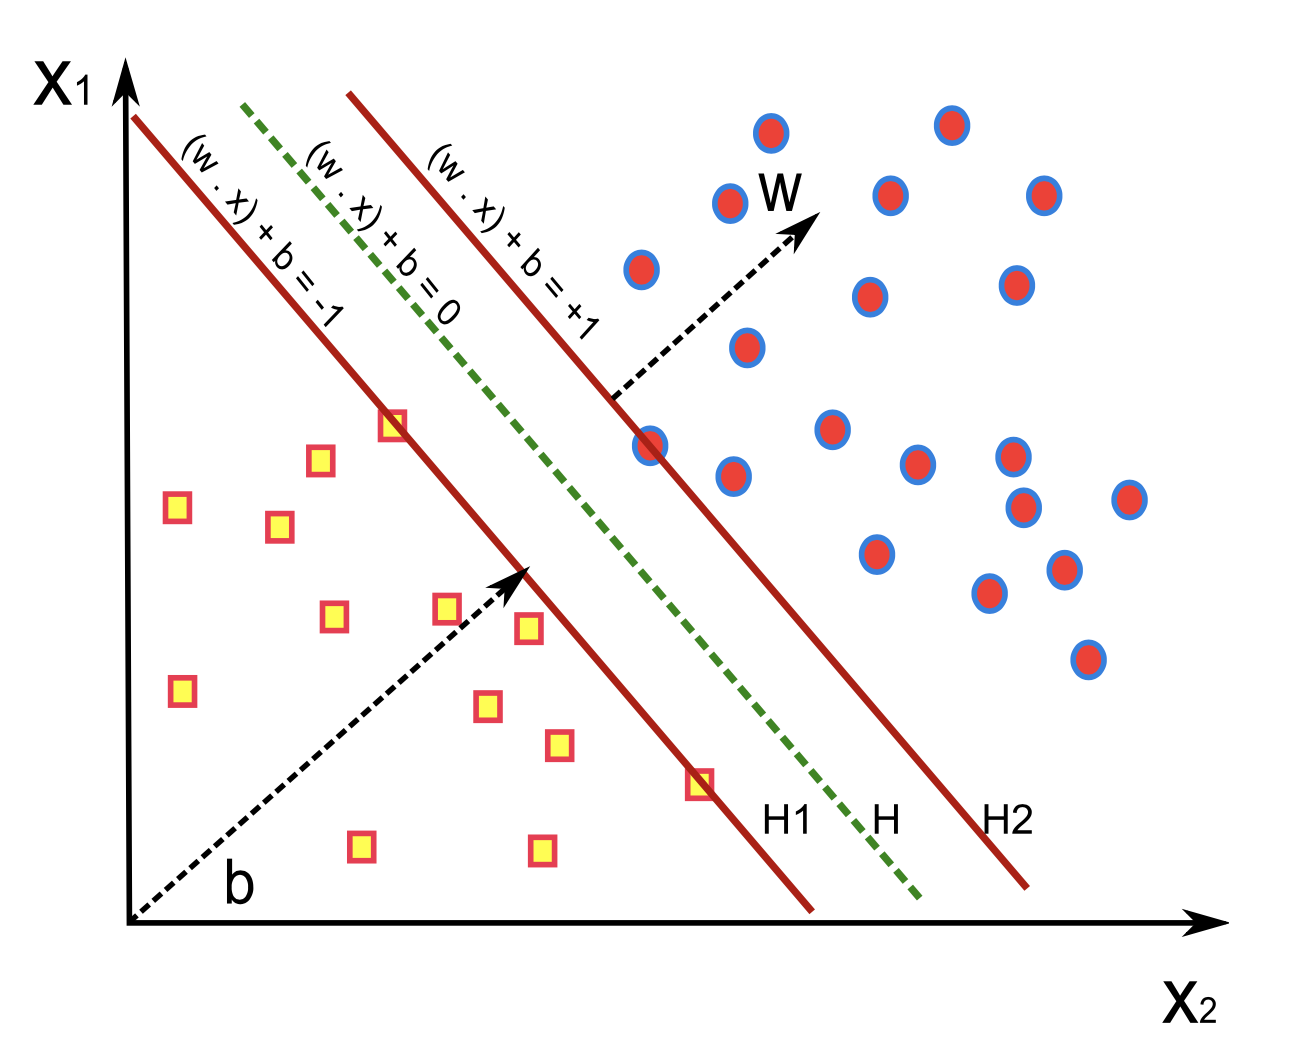
\includegraphics[width=0.6\textwidth]{SVM linearly separable.png}
    \caption{SVM Best Hyperplane in the linearly separable case \cite{cervantesComprehensiveSurveySupport2020}.}
    \label{fig:svm-hyperplane}
\end{figure}

The linearly separable case is rare in real life. Instead, datapoints from one class may seem to mix with the other class at the optimal boundary (Figure \ref{fig:svm-hyperplane-non-linearly-separable}). To still find this optimal boundary, a positive slack factor $\zeta_i$ is introduced and controlled by a parameter $C$ that controls the width of the margin. A lower $C$ allows for a wider margin that may improve generalizability in real life at the cost of more misclassification of the training datatset, whereas a higher $C$ tightens the margin and minimizes the classification errors in the training dataset but may decrease generalizability in real life \cite{cervantesComprehensiveSurveySupport2020}.  

\begin{figure}[ht]
    \centering
    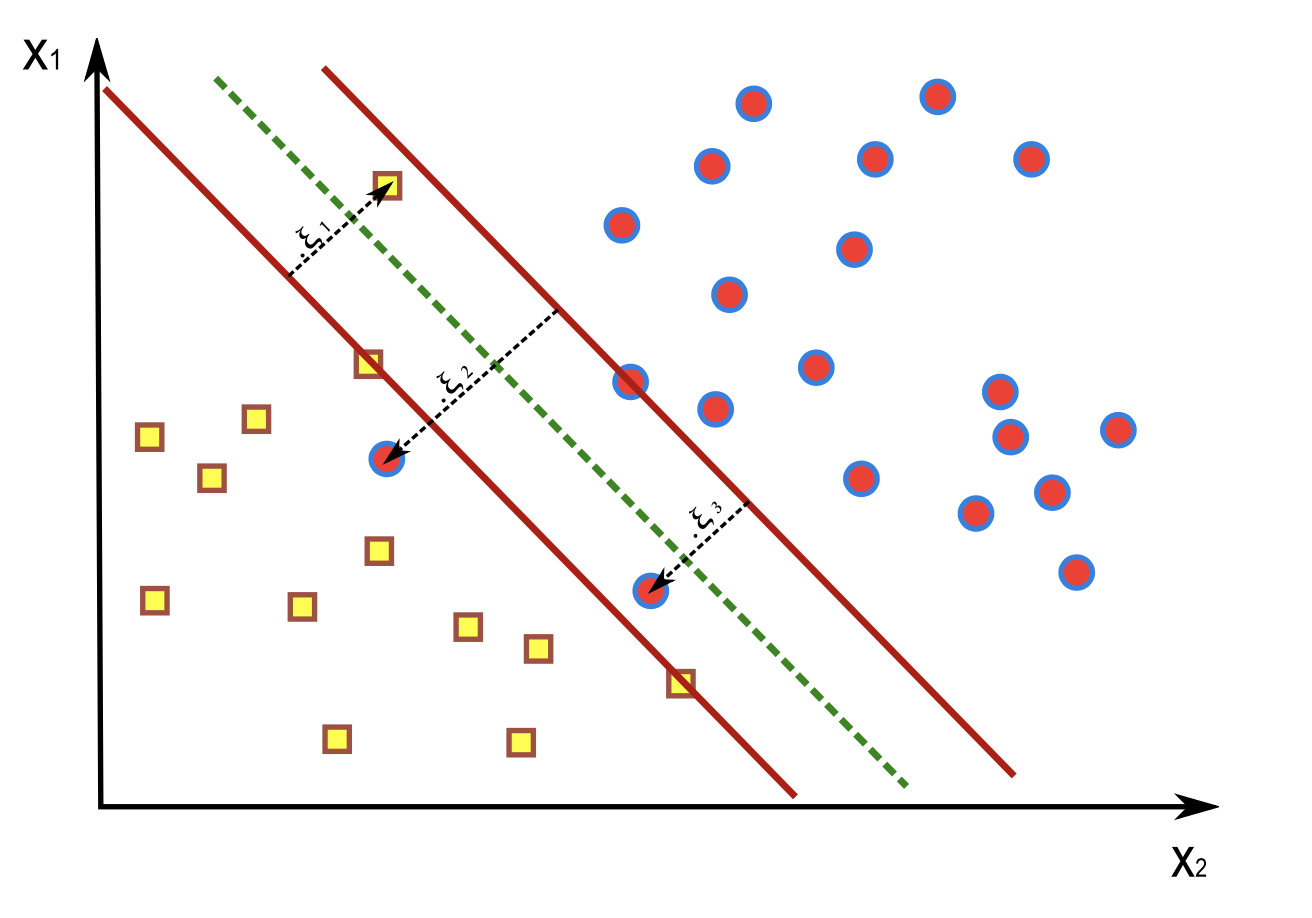
\includegraphics[width=0.6\textwidth]{SVM non-linearly separable.png}
    \caption{SVM Best Hyperplane in the non linearly separable case \cite{cervantesComprehensiveSurveySupport2020}.}
    \label{fig:svm-hyperplane-non-linearly-separable}
\end{figure}

SVM can also be used separate data that is not separable by a linear hyperplane (Figure \ref{fig:svm-hyperplane-non-linearly-classifier}) by using a kernel. Kernels reframe the problem in a highly dimensional space called the "feature space" and in this feature space, it is simple for the algorithm to find the hyperplane. In the next subsection that will detail the convex optimization problem for SVM, it is found that the function that needs to be optimized depends on the inner product between every sample $\langle x_i \cdot x_j \rangle$. Transforming the original dataset to this feature space through a transfer function $\phi$ yields an optimization problem that depends on $\langle \phi(x_i) \cdot \phi(x_j) \rangle$. Kernel functions $K(x_i, x_j)$ are special functions that provide an equivalent way to calculate $\phi(x_i) \cdot \phi(x_j)$ (ie $\phi(x_i) \cdot \phi(x_j) = K(x_i, x_j)$) without having to initially transform the original dataset using $\phi$ since transforming the dataset to the feature space may be a costly operation if there are many features. The following are popular kernels \cite{cervantesComprehensiveSurveySupport2020}:

\begin{enumerate}
    \item Linear Kernel: $K(x_i, x_j) = x_i \cdot x_j$
    \item Polynomial Kernel: $K(x_i, x_j) = (1 + x_i \cdot x_j)^p$
    \item Gaussian Kernel: $K(x_i, x_j) = e^{-\frac{{\left\lVert x_i - x_j\right\rVert}^2}{2\sigma^2}}$
    \item RBF Kernel: $K(x_i, x_j) = e^{-\gamma(x_i - x_j)^2}$
    \item Sigmoid Kernel: $K(x_i, x_j) = tanh(\eta x_i \cdot x_j + v )$
\end{enumerate}

\begin{figure}[ht]
    \centering
    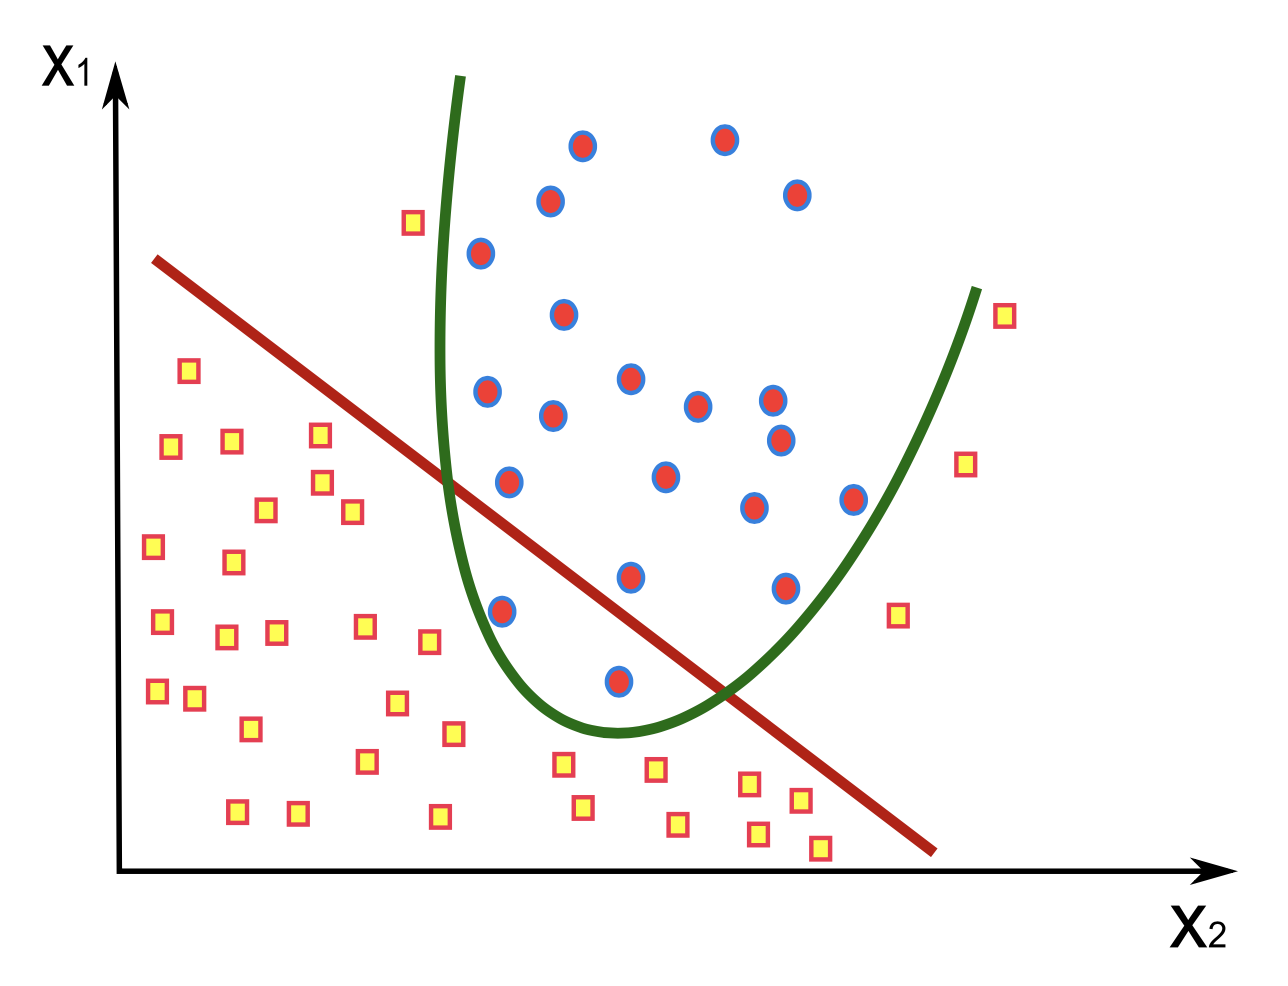
\includegraphics[width=0.6\textwidth]{SVM non-linear classifier.png}
    \caption{SVM non-linear classifier (green line) \cite{cervantesComprehensiveSurveySupport2020}.}
    \label{fig:svm-hyperplane-non-linearly-classifier}
\end{figure}

Since SVM can only separate between 2 classes as a binary classifier, a further step must be done to separate multiple classes. Scikit-learn uses a one vs. rest strategy by default. For each class a decision boundary between itself and the rest of the samples are created. For an unlabeled point a probability of membership to each class is calculated and an argmax function is used to determine the membership \cite{12MulticlassMultioutput}.

\clearpage
\subsubsection{Theory of SVM: Linearly Separable}
Consider a training dataset $X = \{x_i, y_i\}^n_{i=1}$ consisting of $n$ samples of feature vectors $x_i \in \mathbb{R}$ and labels $y_i \in (-1, 1)$. In the linearly separable case of SVM, the two classes in our training dataset can be separated perfectly by a hyperplane. The data labelled with class $y=1$ will be on one side of the hyperplane and the other class $y=-1$ will be on the other side of the hyperplane. The equation for a hyperplane is given in Equation \ref{eq:hyperplane}

\begin{equation}
    \mathbf{w \cdot x} + b = 0
    \label{eq:hyperplane}
\end{equation}

Where $x \in \mathbb{R}^d$, and $\mathbf{w}$ the weights for the hyperplane and $b$ the bias. For simplicity of visualization, consider $x \in \mathbb{R}^2$. The SVM optimization problem tries to find $\mathbf{w}$ and $b$ such that the margin (ie. the distance to the closest point(s) to the hyperplane) is maximized. One variation of this margin called the functional margin $F$ uses the $y_i$ label to ensure that the margin is positive for individual samples correctly classified by some hyperplane with parameters ($\mathbf{w}$, $b$) and is given by the Equation \ref{eq:func_margin}

\begin{equation}
    F = \min_{i=1...n}{[y_i (\mathbf{w} \cdot x_i + b)]}
    \label{eq:func_margin}
\end{equation}

In the SVM optimization problem, this functional margin is set to $F=1$ as shown in \ref{fig:svm-hyperplane} and results in the parallel hyperplanes H1 and H2 as the constraint of the problem (Eq. \ref{eq:svm-constraint}).

\begin{equation}
    y_i (\mathbf{w} \cdot x_i + b) \geq 1 \; \forall \; i
    \label{eq:svm-constraint}
\end{equation}

The goal now is to maximize the distance between the hyperplanes H1 and H2 to obtain the optimal hyperplane H which falls in the middle of H1 and H2. The minimum distance from H to H2 (or H to H1) is called the geometric margin. This minimum distance can be found be taking the vector between any point on H2: $p_{H2}$ and any point on H1: $p_{H1}$ and projecting it onto the unit normal vector of H1 or H2 given by $\mathbf{w}$. Keep in mind that $p_{H2}$ must satisfy $\mathbf{w} \cdot \mathbf{x} + b = 1$ and $p_{H1}$ must satisfy $\mathbf{w} \cdot \mathbf{x} + b = -1$

\begin{equation*}
    \begin{split}
    d &= \left\lVert\text{proj}_\mathbf{w}{(p_{H2} - p_{H1})} \right\rVert \\
     &= \left\lVert \left ((p_{H2} - p_{H1}) \cdot \mathbf{\frac{w}{||w||}}\right ) \frac{\mathbf{w}}{||\mathbf{w}||} \right\rVert \\ 
     &= \left\lVert \left (p_{H2} \cdot \mathbf{w} - p_{H1} \cdot \mathbf{w} \right ) \frac{\mathbf{w}}{||\mathbf{w}||^2} \right\rVert
    \end{split}
\end{equation*}

 $p_{H2}$ must satisfy $\mathbf{w} \cdot p_{H2} + b = 1$ (ie $\mathbf{w} \cdot p_{H2} = b - 1$) to be on hyperplane H2 and $p_{H1}$ must satisfy $\mathbf{w} \cdot p_{H1} + b = -1$ to be on hyperplane H1 (ie $\mathbf{w} \cdot p_{H1} = -b - 1$)

\begin{equation}
    \begin{split}
     &= \left\lVert \left ((1 - b) - (-b - 1) \right ) \frac{\mathbf{w}}{||\mathbf{w}||^2} \right\rVert \\
     &= \left\lVert 2 \frac{\mathbf{w}}{||\mathbf{w}||^2} \right\rVert \\ 
     d &= \frac{2}{||\mathbf{w}||}
    \end{split}
\end{equation}

To find the optimal hyperplane, the distance $d = 2 / ||\mathbf{w}||$ must be maximized or equivalently $||\mathbf{w}||^2$ (which is a convex function \cite{cervantesComprehensiveSurveySupport2020}) can be minimized giving rise to the following convex optimization problem that can be solved using Lagrange Duality. The primal problem is:

\begin{equation}
    \begin{split}
    & \min ||\mathbf{w}||^2 \\
    & \text{s.t.} \; y_i (\mathbf{w} \cdot x_i + b) \geq 1 \; \forall \; i
    \end{split}
    \label{eq:svm-optimization}
\end{equation}

Converting equation \ref{eq:svm-optimization} to the Lagrange Formulation which causes the constraint to move to the objective function and act as a penalty if the constraint is violated:

\begin{equation}
    L(\mathbf{w}, b, \alpha) = \frac{1}{2} \langle \mathbf{w} \cdot \mathbf{w} \rangle - \sum^n_{i=1}{\alpha_i[y_i(\langle \mathbf{w} \cdot x_i \rangle + b) - 1]}
\end{equation}

Setting partial derivatives with respect to $\mathbf{w}$ and $b$ equal to zero to minimize the Lagrangian:

\begin{equation}
    \label{eq:lagrangian-partial-deriv}
    \begin{split}
        \frac{\partial L(\mathbf{w}, b, \alpha)}{\partial \mathbf{w}} = \mathbf{w} - \sum^n_{i=1}{\alpha_i y_i x_i} = 0 & \rightarrow \mathbf{w} = \sum^n_{i=1}{\alpha_i y_i x_i} \\
        \frac{\partial L(\mathbf{w}, b, \alpha)}{\partial b} = - \sum^n_{i=1}{\alpha_i y_i} = 0 & \rightarrow \sum^n_{i=1}{\alpha_i y_i} = 0
    \end{split}
\end{equation}

Substituting these into the Lagrange Formulation and simplifying yields the dual that depends only on the Lagrange Multipliers $\alpha$ \cite{cervantesComprehensiveSurveySupport2020}.

\begin{equation}
    L(\mathbf{w}, b, \alpha) = - \frac{1}{2} \sum_{i=1}^n{\sum_{j=1}^n{\alpha_i y_i \alpha_j y_j \langle x_i \cdot x_j \rangle}} + \sum_{i=1}^n{\alpha_i}
\end{equation}

Then the dual optimization problem is shown in Equation \ref{eq:svm-dual} and the solution to the dual is the same as the solution to the primal given that the Karush-Kuhn-Tucker conditions (KKT) are satisfied \cite{cervantesComprehensiveSurveySupport2020}:

\begin{equation}
    \label{eq:svm-dual}
    \begin{split}
        & \max_{\alpha_i} - \frac{1}{2} \sum_{i=1}^n{\sum_{j=1}^n{\alpha_i y_i \alpha_j y_j \langle x_i \cdot x_j \rangle}} + \sum_{i=1}^n{\alpha_i} \\
        & \text{s.t.} \: \alpha_i \ge 0, \: 1, ..., n \\
        & \: \sum^n_{i=1}{\alpha_i y_i} = 0
    \end{split}
\end{equation}

The solution to the Lagrangian Multipliers $\alpha_i$ can be found using quadratic programming. It is observed that $\alpha_i > 0$ are called the support vectors and all other $\alpha_i = 0$ \cite{cervantesComprehensiveSurveySupport2020}. Once $\alpha_i$ is found, $\mathbf{w}$ can be found using the training data and $\alpha_i$ in Equation \ref{eq:lagrangian-partial-deriv}. Since the support vectors have been found and known to fall on hyperplane H1 and H2, and the normal $\mathbf{w}$ has been found, the optimal $b$ can be found by isolating for $b$ in H2: $(\mathbf{w} \cdot x_{H2}) + b = 1$ or H1: $(\mathbf{w} \cdot x_{H1}) + b = -1$ for a support vector that falls on H2 or H1 respectively.

\subsubsection{Theory of SVM: Not Linearly Separable}


\clearpage
\subsection{Random Forests}

\subsection{Wavelets}

\section{Neural Networks}
\subsection{Deep Nerual Networks}
\subsection{Convultional Neural Networks}
\subsection{Recurrent Neural Networks}
\subsection{Long Short Term Memory}

\section{Large Language Models}

 
\section{Feature Extraction}
Time series data is a series of data that each consists of a value at an associated timestamp. In terms of the system investigated in this thesis, this could be a series of position in the x-axis measured at time $t_1, t_2, t_3...$ respectively. The data can be said to be indexed by time \cite{yinPredictionAnalysisTime2023} typically in ascending order.



\chapter{Pilot Testing of Detecting Activities to make a Sandwich}
Continuing from the findings in Chapter \ref{chp3}, the 9H anchor configuration
was used to perform a preliminary classification of activities in the 
kitchen. Steps performed in making a sandwich were broken down and organized
into Setup, Preparation, Cooking, and Finishing steps, Figure \ref{fig:sandwichbreakdown}. 

\begin{figure}[ht]
    \centering
    \includegraphics*[width=\textwidth]{makingsandwich}
    \caption{Task decomposition of making a sandwich.}
    \label{fig:sandwichbreakdown}
\end{figure}

From the actions shown in Figure \ref{fig:sandwichbreakdown}, actions 
with distinct location or patterns were selected as classes for classification.
OPENFRIDGE, OPENFREEZER, and GETPLATE were selected as classes from the Setup
category, washing hands/vegetables/fruits/using the kitchen sink were grouped 
into a WASHHANDS category, and SLICETOMATO were selected as a class. Finally,
All intermediary transitions or motionless segments were grouped into a 
UNDEFINED category. Single trials were performed to collect data for each of 
these classes. 

\clearpage
\section{Experimental Protocol}
\subsection{Setup}
Several points were enforced to ensure that the training dataset captures
the variation in action sufficiently when classifying data from right-handed individuals.

\begin{itemize}
    \item Pozyx Tag is mounted on the right wrist (Figure \ref{fig:wristsensor}).
    \item Initial position for each of the single trials are not marked. Participant
    will be able to choose a location from which they can perform the action comfortably
    without moving their feet.
    \item An action starts when the individual contacts the appliance or furniture.
    For SLICETOMATO the action starts when an individual starts slicing the 
    tomato and ends when they stop slicing the tomato. Motions such as picking up the
    knife and getting in position to slice were considered transitions and labelled 
    as UNDEFINED. 
\end{itemize}


\begin{figure}[ht]
    \centering
    \includegraphics*[width=0.4\textwidth]{wristsensor}
    \caption{Pozyx tag mounted on the wrist. The participant is performing the 
    OPENFRIDGE task
    }
    \label{fig:wristsensor}
\end{figure}

\subsection{Data Collection}
Custom Python stopwatch scripts were created to accurately label periods of 
transitions (quiet standing + getting into position for the action) and the action.
An example of the data collected is shown in Figure \ref{fig:openfridgedata}. 
For each action there is a quiet standing period at the beginning and end. 
OPENFRIDGE, OPENFREEZER, OPENPLATE, WASHHANDS each had 5 repetitions for each trial.
SLICETOMATO contained 3 slices to conserve the amount of tomato.
Each action had a total of 5 trials. 

\begin{figure}[ht]
    \centering
    \includegraphics*[width=\textwidth]{openfridgedata}
    \caption{Labelled position data of the OPENFRIDGE action. Note that the "quiet standing"
    periods do not consist entirely of quiet standing, but also include traces of 
    transitions from getting into the correct position to perform the action. 
    }
    \label{fig:openfridgedata}
\end{figure}

Since the Pozyx Tag contained a BNO055 chip, in addition to 3D Position data, the
tags were able to capture inertial data including Accelerometer Data, 
Linear Accelerometer Data, Angular Velocity Data, and the orientation.

Data for each of the actions that relate to making a sandwich were collected from 
2 participants.

\section{Feature Extraction}
An initial sliding window with a width of 2 seconds and a stride length of 1 second
was used to ensure that enough feature vectors could be extracted from the SLICETOMATO dataset.
An example of a windows taken for the OPENFRIDGE action and UNDEFINED action 
are shown in Figure \ref{fig:windows}.

\begin{figure}[ht]
    \centering
    \begin{subfigure}{\textwidth}
        \includegraphics*[width=\textwidth]{windowing1}
        \caption{}
    \end{subfigure}
    \begin{subfigure}{\textwidth}
        \includegraphics*[width=\textwidth]{windowing3}
        \caption{}
    \end{subfigure}
    \caption{Obtaining windows from the OPENFRIDGE dataset. The green vertical
    lines section off a 2-second window. (a) A window
    labelled OPENFRIDGE. (b) A window labelled UNDEFINED.
    }
    \label{fig:windows}
\end{figure}

From each window, basic statistical measures over the entire window were taken. These
measures include the MEAN, MEDIAN, MODE (to 5cm for position), MAX, MIN, and STD
of the entire window. 
From each window of data, there were a total of 3 (axes) * 5 (types of data) * 6 (statistical measures) = 90 Features 

From the entire timeseries dataset, 2773 feature vectors were extracted.
Refer to Table \ref{tab:countsfeatvect} for the breakdown of counts for each label.

\begin{table}[!htbp]
  \centering
  \caption{Count of the occurrences of each action.}
  \label{tab:countsfeatvect}
  \begin{tabular}{ll}
    \toprule
    \thead{Action} & \thead{Count} \\
    \midrule
    UNDEFINED   & 1518 \\
    SLICETOMATO & 197 \\
    WAHSHANDS   & 316 \\
    OPENFRIDGE  & 239 \\
    OPENFREEZER & 203 \\
    GETPLATE    & 300 \\
    \bottomrule
  \end{tabular}
\end{table}

\clearpage
\section{Model Selection}
A 60:40 split was used to train and test the model selected. Several models 
were chosen including Linear Support Vector Machine, Radial Support Vector Machine,
K-Nearest Neighbors, Decision Trees and Random Forests. As this was a pilot study in determining the 
feasibility of classification of the fine-grained actions involved
in making a sandwich, rigorous parameter tuning and feature selection 
were neglected and the defaults from the sklearn Python package were used.

\section{Results}
The confusion matrices from each model are output in Figures \ref{fig:cm-svm-lin}-\ref{fig:cm-rf}.
Total accuracy was reported as well as the sensitivity, specificity, and precision of each class 
were reported. These measures are calculated as follows:

\begin{equation}
    \text{Accuracy} = \frac{\text{All} \: TP}{N}
\end{equation}

\begin{equation}
    \text{Sensitivity} = \frac{TP}{TP + FN}
\end{equation}

\begin{equation}
    \text{Precision} = \frac{TP}{TP + FP}
\end{equation}

\begin{equation}
    \text{Specificity} = \frac{TN}{TN + FP}
\end{equation}
Where $N$ is the number of samples $TP$ are True Positives, 
$TN$ are true negatives, $FP$ are false positives and $FN$ are false negatives.

\begin{figure}[ht]
    \centering
    \includegraphics*[height=0.8\textheight]{cm-svm-lin}
    \caption{Test confusion matrix using the Support Vector Classifier with a Linear Kernel}
    \label{fig:cm-svm-lin}
\end{figure}


\begin{figure}[ht]
    \centering
    \includegraphics*[height=0.8\textheight]{cm-svm-rbf}
    \caption{Test confusion matrix using the Support Vector Classifier with a Radial Kernel}
    \label{fig:cm-svm-rbf}
\end{figure}

\begin{figure}[ht]
    \centering
    \includegraphics*[height=0.8\textheight]{cm-svm-poly}
    \caption{Test confusion matrix using the Support Vector Classifier with a Polynomial Kernel}
    \label{fig:cm-svm-poly}
\end{figure}

\begin{figure}[ht]
    \centering
    \includegraphics*[height=0.8\textheight]{cm-5nn}
    \caption{Test confusion matrix using the K-Nearest Neighbors Classifier}
    \label{fig:cm-5nn}
\end{figure}

\begin{figure}[ht]
    \centering
    \includegraphics*[height=0.8\textheight]{cm-decision}
    \caption{Test confusion matrix using the Decision Tree Classifier}
    \label{fig:cm-decision}
\end{figure}

\begin{figure}[ht]
    \centering
    \includegraphics*[height=0.8\textheight]{cm-rf}
    \caption{Test confusion matrix using the Random Forests Classifier}
    \label{fig:cm-rf}
\end{figure}

\clearpage
\section{Discussion}
Table \ref{tab:accuracies} summarizes the accuracies obtained from each model.

\begin{table}[!htbp]
  \centering
  \caption{Accuracy of each Model}
  \label{tab:accuracies}
  \begin{tabular}{ll}
    \toprule
    \thead{Model Name} & \thead{Accuracy (\%)} \\
    \midrule
    SVM Linear      & 97.7 \\
    SVM Radial      & 88.1 \\
    SVM Polynomial  & 93.1 \\
    kNN             & 97.4 \\
    Decision Tree   & 97.5 \\
    Random Forests  & 99.3 \\
    \bottomrule
  \end{tabular}
\end{table}

With the exception of the Radial SVM, all of the models perform well
achieving an accuracy of somewhere in the high 90s. In day-to-day
activities, there is a disproportionately higher number of the 
UNDEFINED class compared to the other "action" classes signifying the 
presence of class imbalance. If a classifier 
guesses all UNDEFINED it can obtain an accuracy of 599/1110 = 54\%. Thus,
accuracies taken around 54\% should be interpreted with caution. Other 
metrics such as the Sensitivity, Precision and Specificity have been provided
to address this class imbalance. Sensitivity is the rate at which the classifier
predicts a $TP$, Precision is the fraction of predictions that are actually
true, and Specificity is the rate at which the classifier predicts a $TN$.
Of all the models, the Random Forests Classifier at the default settings
seem to the best in terms of Accuracy and Precision, Sensitivity, and Specificity
for all classes. 

The performance of these models in the real-time will need to be tested 
and quantified before any conclusions can be made. A high accuracy 
is promising, but may also be indicative of overfitting which means 
that the model will not be able to generalize variation experienced in the 
real world. In later sections, more fine-grained actions will be considered,
models will be more rigorously tuned, and the performance in real-time
will be investigated.



\chapter{PASS Tasks}
% Note when we get to this section we can introduce temporal variation by stretching or shrinking our signals to augment our dataset to get more samples (and simulate potential an older adult).

\section{Selecting Cooking Tasks}
To employ some of the time-series classification methods discussed in Chapter \ref{chp4}, a dataset of the proposed positional + IMU system is required. Chapter \ref{chp2}'s section on the traditional assessments of ADLs will serve as a basis for the selection of tasks to perform and collect data from. Of the assessments discussed, Table \ref{tab:cooking-task-summary} summarizes the assessments with cooking tasks mentioned in its procedure.

\begin{table}[ht]
    \small
    \centering
    \caption{Cooking tasks in the Assessment tools for the IADLs.}
    \label{tab:cooking-task-summary}
    \renewcommand{\arraystretch}{1.5}
    \begin{tabularx}{\textwidth}{>{\hsize=.8\hsize}X X }
        \hline
        \textbf{Tool} & \textbf{Tasks} \\
        \hline
        PASS & making soup with water/milk \\
        & making muffins in the oven \\
        & cutting up fruit \\
        Self-Assessment PD Disability Scale & making a cup of tea \\
        & inserting electrical plug \\
        & pouring milk from bottle \\
        & opening tins \\
        & washing \\
        Melbourne Low-vision ADL Index & preparing meals \\
        Lawton Instrumental ADL Scale & plans, prepares and serves adequate meals independently \\
        Frenchay Activities Index & preparing main meals \\
        Texas Functional Living Scale & Describe how to make peanut butter and jelly sandwich \\
        \hline
    \end{tabularx}
\end{table}

Of the assessments in Table \ref{tab:cooking-task-summary}, the cooking task(s) in the Melbourne Low-vision ADL Index, Lawton Instrumental ADL Scale, Frenchay Activities Index, and Self-Assessment PD Disability Scale are all questionnaires and as a result do not have concrete steps on how the task should be performed. Futhermore, the Melbourne Low-vision ADL Index, Lawnton Instrumental ADL Scale and the Frenchay Activities Index only have general requirements for the cooking task such as the ability to "prepare meals," and "plans, prepares and serves adequate meals independently." These general cooking tasks may be useful in the evaluation of ADL ability in a questionnaire format by requesting the older adult to holistically consider their ability to cook, but may not be the best candidates when looking for fine-grained actions to extract. 

The remaining 2 assessment tools, the Texas Functional Living Scale and Performance Assessment of Self-Care Skills (PASS), mention cooking task(s) that requires a clinician to evaluate. Upon closer inspection of the Texas Functional Living Scale, however, the individual is only required to describe the task and not actually perform it. The only candidate that has clear cooking tasks broken down into their fine-grained actions is the PASS and will be used as a reference for the experiment protocol and extraction of fine-grained tasks. 3 Cooking Scenarios are presented in the PASS: making soup with water/milk, making muffins in the oven, and cutting up fruit. The 3 cooking scenarios are shown in Figures \ref{fig:PASS-muffin}-\ref{fig:PASS-soup}.

\begin{figure}[ht]
    \centering
    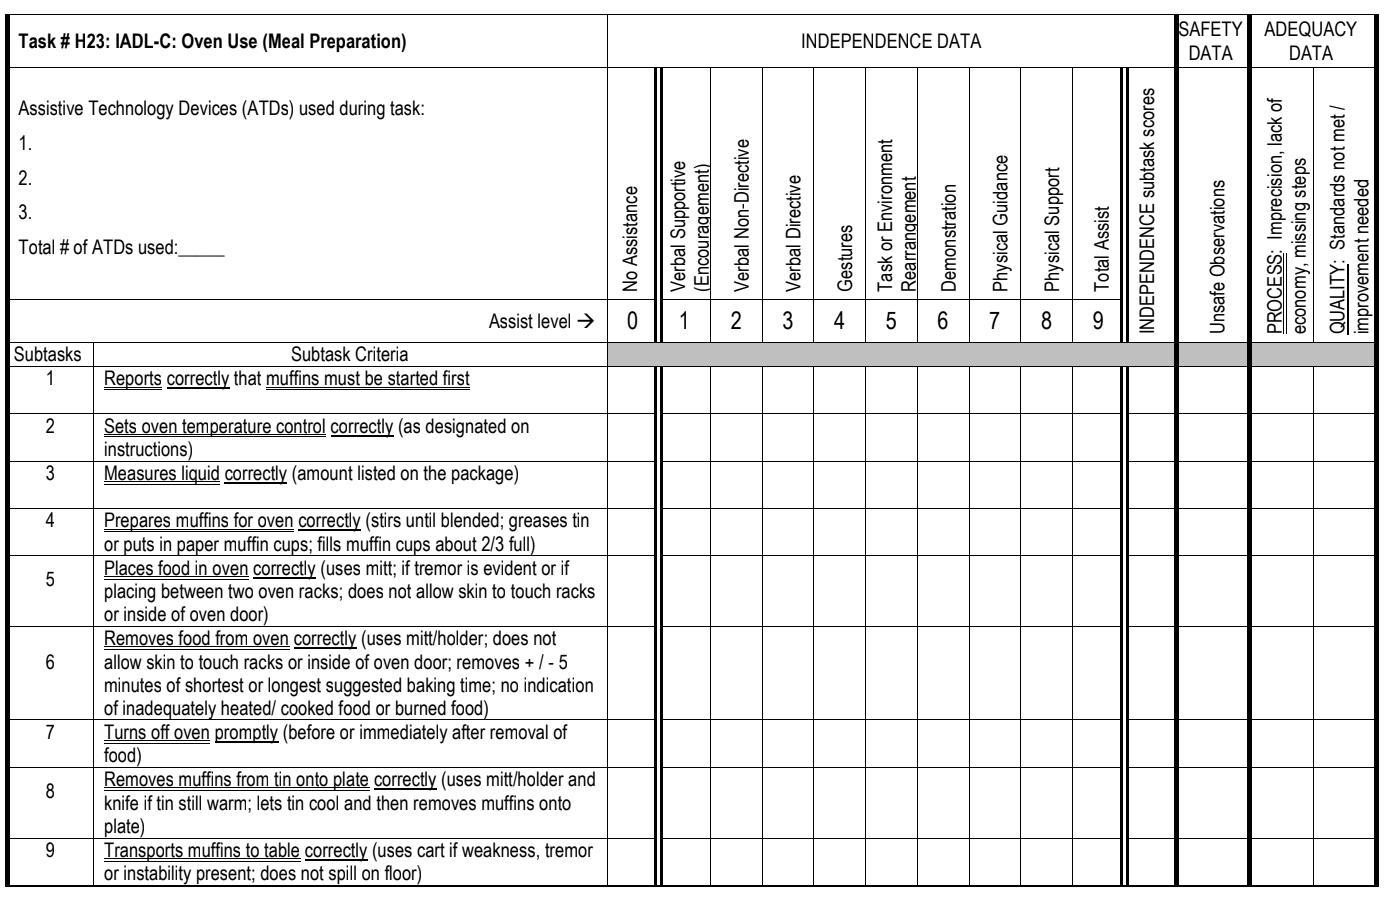
\includegraphics[width=0.95\textwidth]{pass-muffin.png}
    \caption{PASS Muffin Task \cite{rogers_performance_2014}}
    \label{fig:PASS-muffin}
\end{figure}


\begin{figure}[ht]
    \centering
    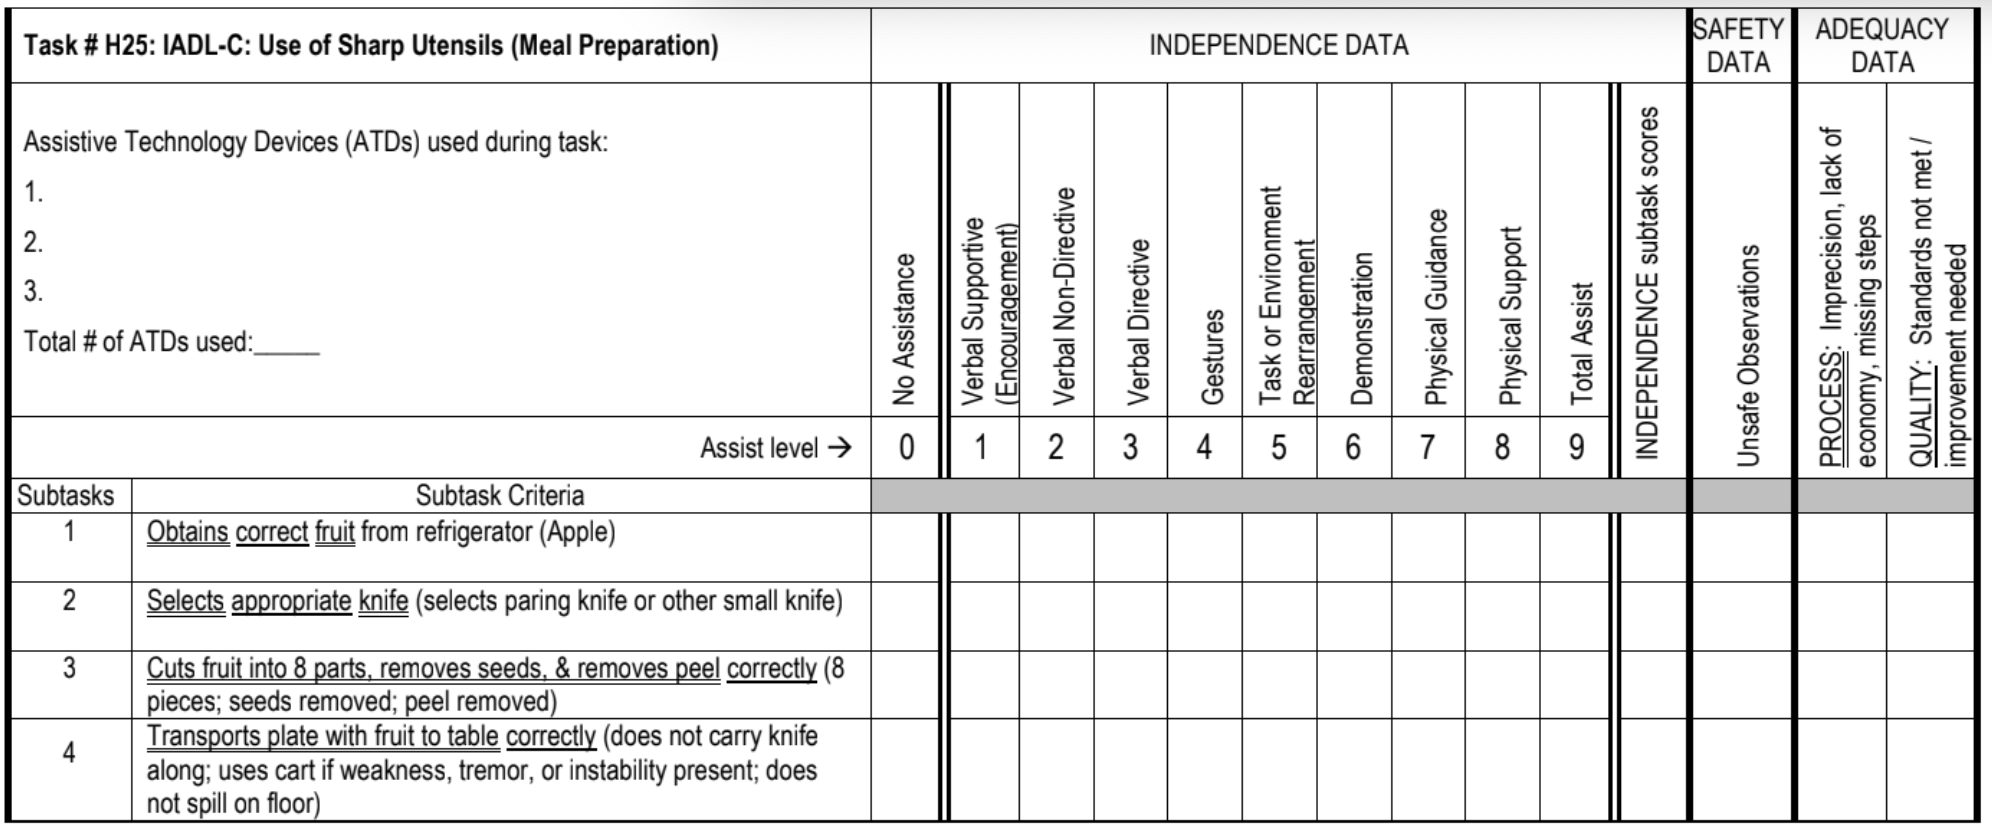
\includegraphics[width=0.95\textwidth]{pass-fruit.png}
    \caption{PASS Fruit Task \cite{rogers_performance_2014}}
    \label{fig:PASS-fruit}
\end{figure}

\begin{figure}[ht]
    \centering
    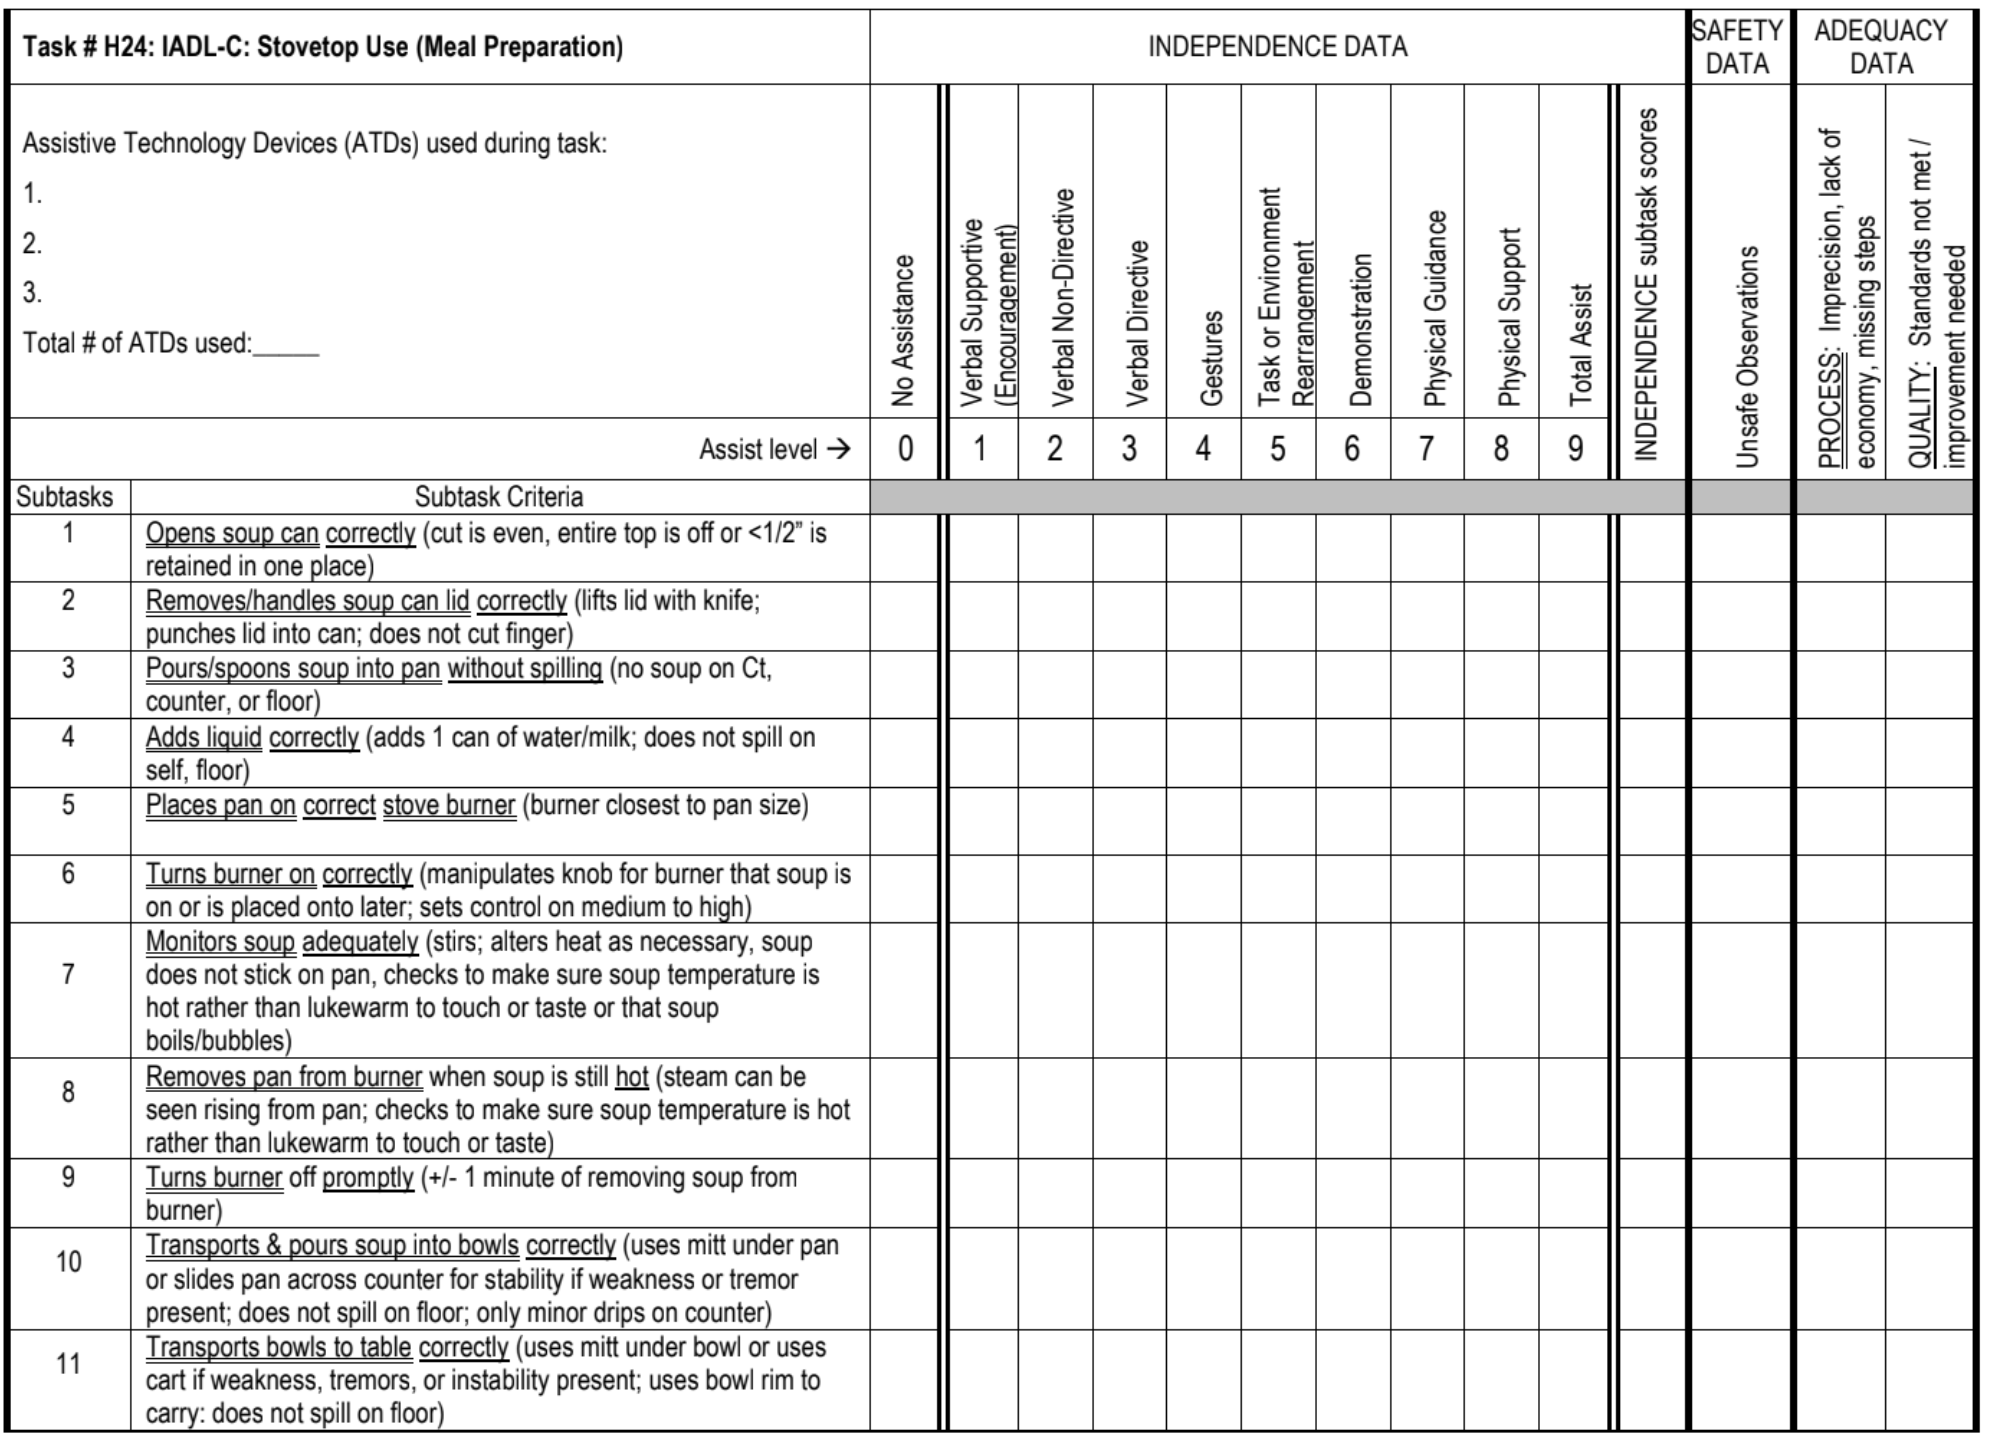
\includegraphics[width=0.95\textwidth]{pass-soup.png}
    \caption{PASS Soup Task \cite{rogers_performance_2014}}
    \label{fig:PASS-soup}
\end{figure}

\section{Fine-grained Task Extraction}
The detail in which tasks can be broken down varies in literature. Human actions may be decomposed all the way into action primitives which is a body part + some motion (eg. right/left hand forward/backward) \cite{huszHumanActivityRecognition2007}. Fine-grained actions can be thought as being one level "coarser" than these action primitives and may combine action primitives to perform a small task (eg. cutting fruit, stir-frying, washing a fruit)  \cite{pan_fine-grained_2020}. A "coarser" level above fine-grained actions are coarse-grained actions and describe the activity that encompasses all of the fine-grained actions (eg. cooking, working). Although action primitives may be useful to consider when breaking down a task, the focus of the thesis is the evaluation of function and ability to perform tasks toward some goal. The detection of coarse-grained actions or activities have been successful in literature previously \cite{cook_learning_2010}, but these coarse-grained actions are too general and do not provide insight into the functional quality of the cooking task. Thus, the focus of the task extraction will be at the "fine-grained" level. 

For each cooking activity in the PASS, an experimental protocol will be developed based on the subtasks outlined in the task document. Although the PASS presents general steps to complete the task, there may sometimes be other actions, or "side-actions" involved in the task. For example, for the Cutting Fruit task in Figure \ref{fig:PASS-fruit}, obtaining the fruit from the refrigerator would require the individual to perform OPEN\_FRIDGE, GRAB\_FRIDGE, and CLOSE\_FRIDGE. The experimental protocol will be more detailed with steps detailing the actions in the PASS as well as any side-actions that occur. Then, from the steps in the experimental protocol, the fine-grained actions can be extracted.




% --------------------------------------------------
% \appendix
% \chapter{Appendix}
% \input{chapters/appendix}

\bibliographystyle{IEEEtran}
\bibliography{ReHM}
\end{document}
